%%% LaTeX Template: Article/Thesis/etc. with colored headings and special fonts
%%%
%%% Source: http://www.howtotex.com/

\documentclass[12pt]{article}


\usepackage{apuntes-estilo}
\usepackage{fancyhdr,lastpage}
\usepackage{color,colortbl}
\usepackage{float}
%\usepackage[dvips]{graphicx}

\def\maketitle{

% Titulo 
\makeatletter
{\color{bl} \centering \huge \sc \textbf{
Ofimática\\
 \vspace*{8pt} }\par}
 \makeatother


% Autor
 \makeatletter
 {\centering \small 
 	Departamento de Ingeniería de Computadoras \\
 	Facultad de Informática - Universidad Nacional del Comahue \\
 	\vspace{20pt} }
 \makeatother

}

% Custom headers and footers
\fancyhf{} % clear all header and footer fields
\fancypagestyle{plain}{\fancyhf{}}
  	\pagestyle{fancy}
 	\lhead{\footnotesize Ofimática - Departamento de Ingeniería de Computadoras}
 	\rhead{\footnotesize \thepage\ }	% "Page 1 of 2"

\def\ti#1#2{\texttt{#1} & #2 \\ }

\begin{document}

\thispagestyle{empty}
\maketitle
\setlength{\parindent}{0pt}


\section*{Introducción}

En la mayoría de las oficinas, sean estas correspondientes a empresas, organismos gubernamentales o simplemente particulares, suelen utilizarse diversas herramientas informáticas con la finalidad de facilitar todas las tareas que se realizan.

Es por esta razón que quienes hacen este tipo de tareas deben estar correctamente capacitados en todas las aplicaciones que sean necesarias para un buen desempeño dentro de la organización. Por otro lado, es necesario que el informático encargado de sistemas, conozca las mejores aplicaciones para que luego pueda recomendar y adiestrar en el uso de las mismas. Además dado que las todas las herramientas ofimáticas que se utilizan en las oficinas suelen actualizarse permanentemente, es importante que quienes estén encargados de utilizarlas también actualicen sus conocimientos.


\section*{Qué es la Ofimática}

En primer lugar vamos a definir qué se entiende por Ofimática. Se llama Ofimática “al conjunto de técnicas, aplicaciones y herramientas informáticas que se utilizan en funciones de oficina para optimizar, automatizar, y mejorar tareas y procedimientos relacionados”\footnote{http://es.wikipedia.org/wiki/Ofimática}.

Usando herramientas informáticas se puede crear, manipular, transmitir o almacenar la información necesaria en una oficina. Por otro lado, hoy en día la ofimática además requiere el uso de redes locales o de Internet, para que los usuarios puedan transmitir datos, correos electrónicos, etc.

\section*{Herramientas Informáticas de Ofimática}

La ofimática surgió ante la necesidad de mecanizar las tareas que se desarrollaban en una oficina. Entonces aparecieron las máquinas de escribir y las fotocopiadoras. Aunque esto supuso un avance, la automatización se incrementó cuando aparecieron las computadoras personales. Entonces empezaron a surgir aplicaciones con un procesador de texto, agenda, calculadora, etc. 

Hoy en día, entre las herramientas informáticas que podemos encontrar hay:
\begin{itemize}
\item Procesadores de texto.
\item Planillas de cálculo.
\item Herramientas de presentación multimedia.
\item Base de datos.
\item Utilidades: agendas, calculadoras, etc.
\item Programas de correo electrónico, correo de voz, mensajeros.
\item Herramientas de reconocimiento y síntesis del habla.
\item Suite ofimática: paquete integrado de aplicaciones ofimática que se distribuyen en conjunto. 
\end{itemize}

Todas estas herramientas están disponibles para su uso en una PC y el producto de las mismas se guardan en unidades de almacenamiento, tales como discos duro, pendrive, etc. Sin embargo, como consecuencia del uso de Internet y el correo electrónico, han ido apareciendo nuevas soluciones ofimáticas basadas en cloud\footnote{http://es.wikipedia.org/wiki/Computacion\_en\_la\_nube}, las cuales ofrecen como ventajas, la accesibilidad a la documentación desde cualquier PC o dispositivo, facilita la cooperación en la edición de la información y minimiza los riesgos de pérdida de datos por robo o ruptura del dispositivo. Entre estas soluciones podemos mencionar Google Drive, Zoho\footnote{https://www.zoho.com/docs/} y ThinkFree Cloud Office\footnote{http://www.thinkfree.com/main.jsp}.

\section*{Suites Ofimática}

Una suite ofimática es un conjunto de aplicaciones utilizadas en oficinas y que permite contar con distintas funcionalidades. La mayoría en general incluye como mínimo un procesador de texto y una hoja de cálculo, pero algunas también incluyen una aplicación para realizar presentaciones,  un sistema de gestión de bases de datos, alguna herramienta básica para gráficos, e incluso aplicaciones para gestionar el correo electrónico y  la agenda.

Dentro de las suites propietarias se encuentra Microsoft Office. La primera versión fue lanzada en 1989 para incorporarla al primer Macintosh que desarrolló la empresa Apple. Luego, en 1990 apareció Microsoft Office para el sistema operativo Microsoft Windows. Esta primera versión contenía un procesador de textos (Microsoft Word), una hoja de cálculo (Microsoft Excel) y una aplicación para presentaciones (Microsoft PowerPoint). Esta versión se podía completar con la “versión profesional” que tenía una aplicación de bases de datos (Microsoft Access) y un gestor de información personal (Microsoft Schedule Plus) que más tarde se convertiría en lo que hoy conocemos como Microsoft Outlook.

Con el paso del tiempo, mientras Microsoft Office evolucionaba, comenzó el desarrollo de otra suite ofimática propietaria llamada StartOffice, perteneciente a la empresa StarDivision. Esta suite fue importante, ya que se convirtió en el punto de inicio de las herramientas libres de oficina. 

En 1999, la empresa Sun Microsystem adquirió a StarDivision y en el año 2000 liberó su código\footnote{http://www.openoffice.org/press/sun\_release.html} fuente bajo las licencias GNU GPL (General Public License), formando así la base para la suite de código abierto OpenOffice.org. Luego en 2010, Oracle compra Sun Microsystem y de ahí en adelante, como consecuencia de las decisiones que tomó la empresa con respecto al software, la mayoría del equipo de desarrollo de software decidió formar una organización sin fines de lucro llamada The Document Foundation y comenzó el desarrollo de LibreOffice a partir del código liberado de OpenOffice. Finalmente, Oracle donó la suite a Apache Software Foundation, una organización sin fines de lucro. De ahí que el nombre actual de la suite sea Apache OpenOffice\footnote{https://www.openoffice.org/es/}. 

Otras suites ofimáticas libres que surgieron fueron KOffice\footnote{http://es.wikipedia.org/wiki/KOffice} y GNOME Office. KOffice se lanzó por primera vez como parte de KDE2.0 para distribuciones Linux. A mediados de 2010, por desacuerdos entre los desarrolladores principales, la comunidad KOffice se dividió en dos comunidades separadas, KOffice y Calligra\footnote{http://es.wikipedia.org/wiki/Calligra\_Suite}. Actualmente se ha discontinuado el desarrollo de KOffice mientras que Calligra Suite está vigente.

Por otro lado Gnome Office es una suite desarrollada por el proyecto libre GNOME. Es una suite especial porque además incluye aplicaciones que han adoptado pero que no han sido desarrolladas por ellos, tal como Gimp.  

Otra suite que podemos mencionar es IBM Lotus Symphony\footnote{http://es.wikipedia.org/wiki/IBM\_Lotus\_Symphony}, cuyo desarrollo basado en OpenOffice tuvo varias mejoras aportadas por IBM. Pero en 2011 esta variante se reintegró en el código de OpenOffice ya que IBM donó el código fuente de IBM Lotus Symphony al proyecto OpenOffice de la Fundación Apache. 

\subsection*{Apache OpenOffice}

Apache OpenOffice es una suite de oficina de código abierto que ofrece herramientas para el procesamiento de palabras, hojas de cálculo, presentaciones, gráficos, bases de datos y más. La versión 4.1.1 está disponible bajo la Licencia Apache 2.0 \footnote{http://www.apache.org/licenses/LICENSE-2.0.html}, la cual permite descargar gratuitamente de Internet, copiar y redistribuir el software.   

Actualmente hay una comunidad trabajando en el desarrollo de OpenOffice, por lo cual podemos encontrar versiones actualizadas y mejoradas del mismo.

Por otro lado, existen versiones para varios idiomas y la versión de la que hablaremos (4.1.1) es compatible con los sistemas Windows (32 bits), GNU/Linux (32 y 64 bits) y Mac OS X. Esto representa una ventaja ya que es posible editar los documentos en un entorno distinto al de creación del mismo.


En cuanto al formato predeterminado, la suite utiliza el OpenDocument (ODF), un formato de archivo abierto para el almacenamiento de documentos ofimáticos, que además es un estándar a nivel internacional. Un archivo con este formato es un archivo comprimido en un contenedor ZIP, que contiene varios archivos y directorios. Los documentos ODF tienen las siguientes extensiones:
\begin{itemize}
\item *.odt (documentos de procesador de textos)
\item *.ods (documentos de libros de hojas de cálculo)
\item *.odp (documentos de presentaciones)
\item *.odb (documentos de base de datos)
\item *.odg (documento de la aplicación de dibujo vectorial)
\end{itemize}

Sin embargo, además de este formato, OpenOffice permite trabajar con otros formatos\footnote{https://wiki.openoffice.org/wiki/Documentation/OOo3\_User\_Guides/Getting\_Started/File\_formats}. Tiene un gran porcentaje de compatibilidad con Microsoft Office, por lo que los documentos de texto, las hojas de cálculo y las presentaciones de MS Office se pueden abrir, editar y guardar de manera satisfactoria con OpenOffice. La suite también permite guardar documentos en formatos tales como RTF, TXT, Microsoft Office XML y OpenOffice.org XML. Adicionalmente puede exportar documentos directamente al formato PDF y exportar presentaciones al formato Adobe Flash (SWF). OpenOffice.org también cuenta con la capacidad de importar documentos en modo de «sólo lectura» en los formatos Unified Office Format, Data Interchange Format y los formatos propios de Microsoft Works, WordPerfect, Lotus 1-2-3, entre otros.

La suite consta de las siguientes aplicaciones\footnote{https://www.openoffice.org/es/producto/index.html}:
\begin{itemize}
\item Writer: un procesador de textos.
\item Calc: hoja de cálculo.
\item Draw: editor de dibujos y gráficos.
\item Impress: editor de presentaciones multimedia.
\item Base: permite la manipulación completa de base de datos
\item Math: editor de fórmulas matemáticas.
\end{itemize}

\subsubsection*{Interfaz gráfica}

Todas las aplicaciones que componen la suite, comparten muchas características en su interfaz gráfica\footnote{https://wiki.openoffice.org/wiki/ES/Manuales/GuiaAOO/UI}. Veremos alguna de ellas, sin entrar en demasiado detalle. Entre los elementos básicos podemos encontrar los siguientes:

\begin{itemize}
\item Menú principal: todas las aplicaciones tienen una estructura de menú principal semejante. En este menú se encuentran todas las funciones principales del programa, tales como crear un nuevo archivo, imprimir, dar formato al documento, la configuración del programa, etc.

\begin{figure}[H]
\centering
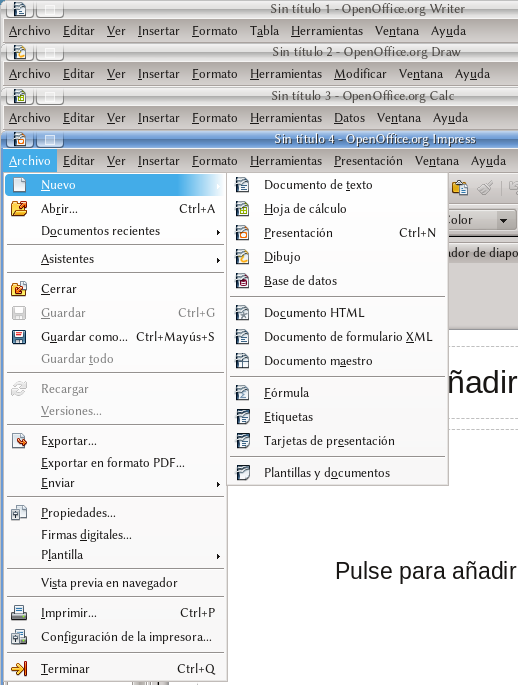
\includegraphics[width=0.8\textwidth]{menuAppsOO.png}
\renewcommand{\figurename}{Fig.}
\caption{Menú principal en aplicaciones de Apache OpenOffice}
\label{contexto:figura}
\end{figure}

\item Menú contextual: realizando con un clic derecho sobre un elemento del documento que se está revisando o sobre un elemento de la interfaz de usuario del programa, se presentará un menú con acciones relativas al elemento seleccionado. Por ejemplo, con un clic derecho sobre una palabra mal escrita se ofrecerán las opciones del corrector ortográfico, mientras que un clic derecho sobre una barra de herramientas permitirá acceder a las opciones de personalización de la misma.

\item Barras de herramientas: una barra de herramientas es un elemento gráfico que contiene varios iconos los cuales permiten activar rápidamente distintas funciones del programa. Algunos de estos iconos ofrecen menús desplegables, otros muestran texto mientras que otros ofrecen funciones directas, como salvar el documento actual, etcétera.

\begin{figure}[h]
\centering
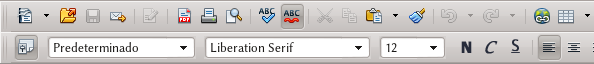
\includegraphics[width=0.8\textwidth]{barraHerramientaOO.png}
\renewcommand{\figurename}{Fig.}
\caption{Ejemplo Barra de herramientas en Apache OpenOffice Writer}
\label{contexto:figura}
\end{figure}

La lista de todas las barras de herramientas disponibles, se encuentra en el menú Ver → Barras de Herramientas. En este menú es posible activar barras que no son visibles como así también desactivar barras presentes en la interfaz.

Existen dos tipos de barras de herramientas: las «normales» que una vez activadas siempre se muestran y las «contextuales» que solo se muestran cuando se selecciona un objeto sobre el cual las herramientas de esa barra aplican. Ejemplo de barras contextuales son las de numeración y viñetas y la de edición de tablas en Writer, la barra de las propiedades de una imagen, la de las propiedades de un objeto gráfico (líneas, cuadros...), etc.

\item Barra de estado: en la parte inferior de la ventana de la aplicación, se puede encontrar información sobre el documento. Por ejemplo, en Writer es posible ver, de izquierda a derecha: el número de página actual, el estilo de página, el idioma del texto en el que se encuentra el cursor, la modalidad del cursor (INSERT para insertar texto normalmente, un clic cambia a SOBRE que sobrescribe el texto), el modo de selección (STD para estándar, EXT para «extendido»...) ... mientras que a la derecha de la barra se encuentra la herramienta para controlar la escala del documento (si se ve al 100 \% o más, si se muestran dos páginas simultáneamente o solo una...)

\item Barra lateral: a partir de Apache OpenOffice 4.0 se introdujo la Barra lateral como un nuevo elemento elemento en la interfaz gráfica que facilita el acceso a las distintas herramientas ofrecidas por cada componente. En la siguiente captura, se la observa a la derecha:

\begin{figure}[H]
\centering
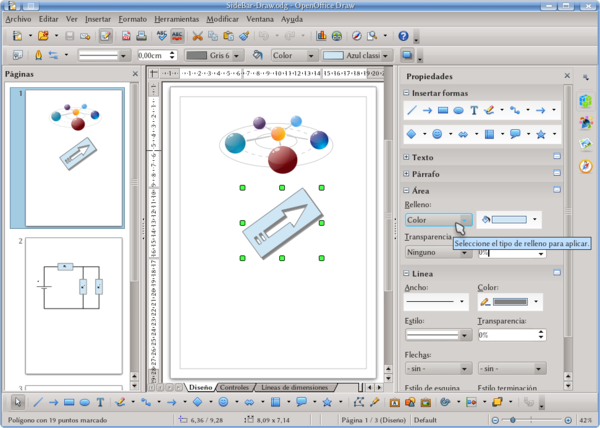
\includegraphics[width=0.8\textwidth]{barraLateralDrawOO.png}
\renewcommand{\figurename}{Fig.}
\caption{Ejemplo Barra lateral en Apache OpenOffice Writer}
\label{contexto:figura}
\end{figure}

\end{itemize}

\subsubsection*{Configuración}
%https://www.openoffice.org/es/soporte/documentacion.html#guiainicio

\subsubsection*{Uso de extensiones para agregar funcionalidad}

\subsubsection*{Uso de estilos y plantillas}

\subsubsection*{Correctores ortográficos}

\subsubsection*{Uso de formatos privativos}

\subsubsection*{Apache OpenOffice Portable}



\subsection*{LibreOffice}

Tal como se mencionara anteriormente, LibreOffice es una suite libre y gratuita, derivada de OpenOffice.org. Esta suite contiene un procesador de texto (Writer), presentaciones en diapositivas (Impress), una planilla de cálculo (Calc), un gestor de base de datos (Base), un programa de diseño de gráficos vectoriales (Draw) y un editor de fórmulas matemáticas (Math). 
Esta suite es multiplataforma, por lo cual puede usarse en sistemas Windows, GNU/Linux y Mac OS X.

Esta suite es la que ha recibido el apoyo de la Free Software Foundation por sobre OpenOffice, porque se distribuye con una licencia GPL totalmente libre. Aunque la FSF reconoce a OpenOffice como una parte importante dentro del ecosistema del software libre, el problema radica fundamentalmente en que se distribuye bajo los términos de la Licencia Apache\footnote{http://es.wikipedia.org/wiki/Apache\_License}. Esta licencia de software libre es sin copyleft, con lo cual alguien podría redistribuirlo de manera comercial. Por ello, la FSF presenta a LibreOffice como una alternativa que permite a los usuarios trabajar con una suite ofimática, protegiendo sus libertades.   

\subsubsection*{LibreOffice portable}

\subsection*{Gnome Office}



\section*{Licencia}
Copyright (C) 2014 Claudia Rozas, Miriam Lechner.

Se concede autorización para copiar, distribuir y/o modificar este documento
bajo los términos de la Licencia Creative Commons Atribución-CompartirDerivadasIgual 3.0 Unported. 

http://creativecommons.org/licenses/by-sa/3.0/
\end{document}

